\subsection{Coordinate specifications}
\begin{tabular}[]{p{0.1\textwidth}p{0.1\textwidth}l}
&&library needed\\
$(x,y)$&Cartesian coordinates&\\
($\theta$:r)&polar coordinates&\\
\verb |($(A)+{sin(60)}*(B)$)|         &coordinate calculations&calc\\
\verb |($(A)!.25!(B)$)|&                 partway calculations&calc\\
\verb |($(A)!3cm!(B)$)|&                 3~cm from (A) in direction of (B)&calc\\
\verb |($(A)!1.2!30:(B)$)|&              stretch by 1.2, then rotate by 30$^{\circ}$&calc\\
\verb |($(A)!(B)!(C)$)|&                 projection of point B onto line AC&calc\\
\verb |($(A)!(B)!30:(C)$)|&              project B onto line AC, then rotate by 30$^{\circ}$&calc\\
\verb '(n1-|n2)'& projection of n2 on the line passing through n1\\
\verb '(n1|-n2)'& projection of n1 on the line passing through n2\\
\verb |\node[above=1cm of| \verb|somenode.north]|&position new node 1~cm above existing anchor&positioning\\
\end{tabular}
\subsubsection{Absolute positioning on the page}
\begin{verbatim}
\begin{tikzpicture}[remember picture, overlay]
  \node [] (node1) at (current page.west) {};
\end{tikzpicture}
\end{verbatim}
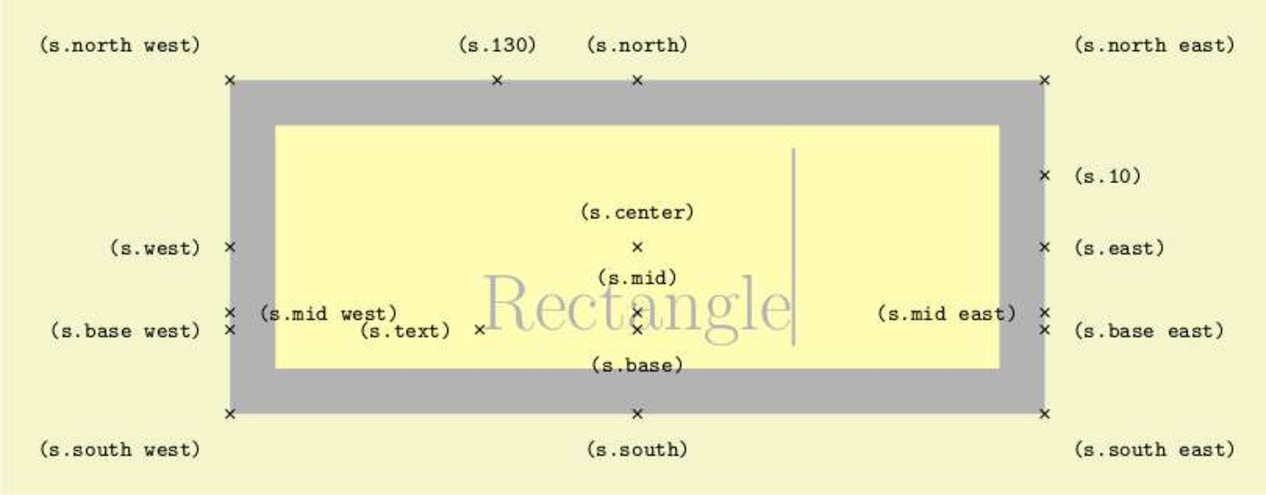
\includegraphics[width=0.33\textwidth]{figures/rectangle_shape.pdf}

\subsection{General}
\verb|\coordinate (X) at (3,5);| name a point X\\
\verb|\node[options] (X) at (3,5) {};| place a node and name it X\\

\subsection{Node options}
\verb |node font=\tiny|\\
\verb 'align=left|center|right' (handling carriage return in nodes)
\verb |text=blue| text color
